% Appendix for TBP chapter
\label{appendix:TBP}
%%%%%%%%%%%%%%%%%%%%%%%%%%%%%%%%%%%%%%%%%%%%%%%%%%%%%%%%%%%%%%%%%%%%%%%%%%%%%%%%%%
%%%%%%%%%%% TBP on Ag(100) @ RT - single ordered island
\paragraph{Ordered areas}
Only a single ordered area of TBP on Ag(100) was found, but its structure could not be resolved properly due to tip issues (compare figure \ref{fig:hex-TBP-Ag100}). Its unit cell looks hexagonal with roughly \SI{1.7} {\nano \meter} period. 

\begin{figure}[h]
	\centering
	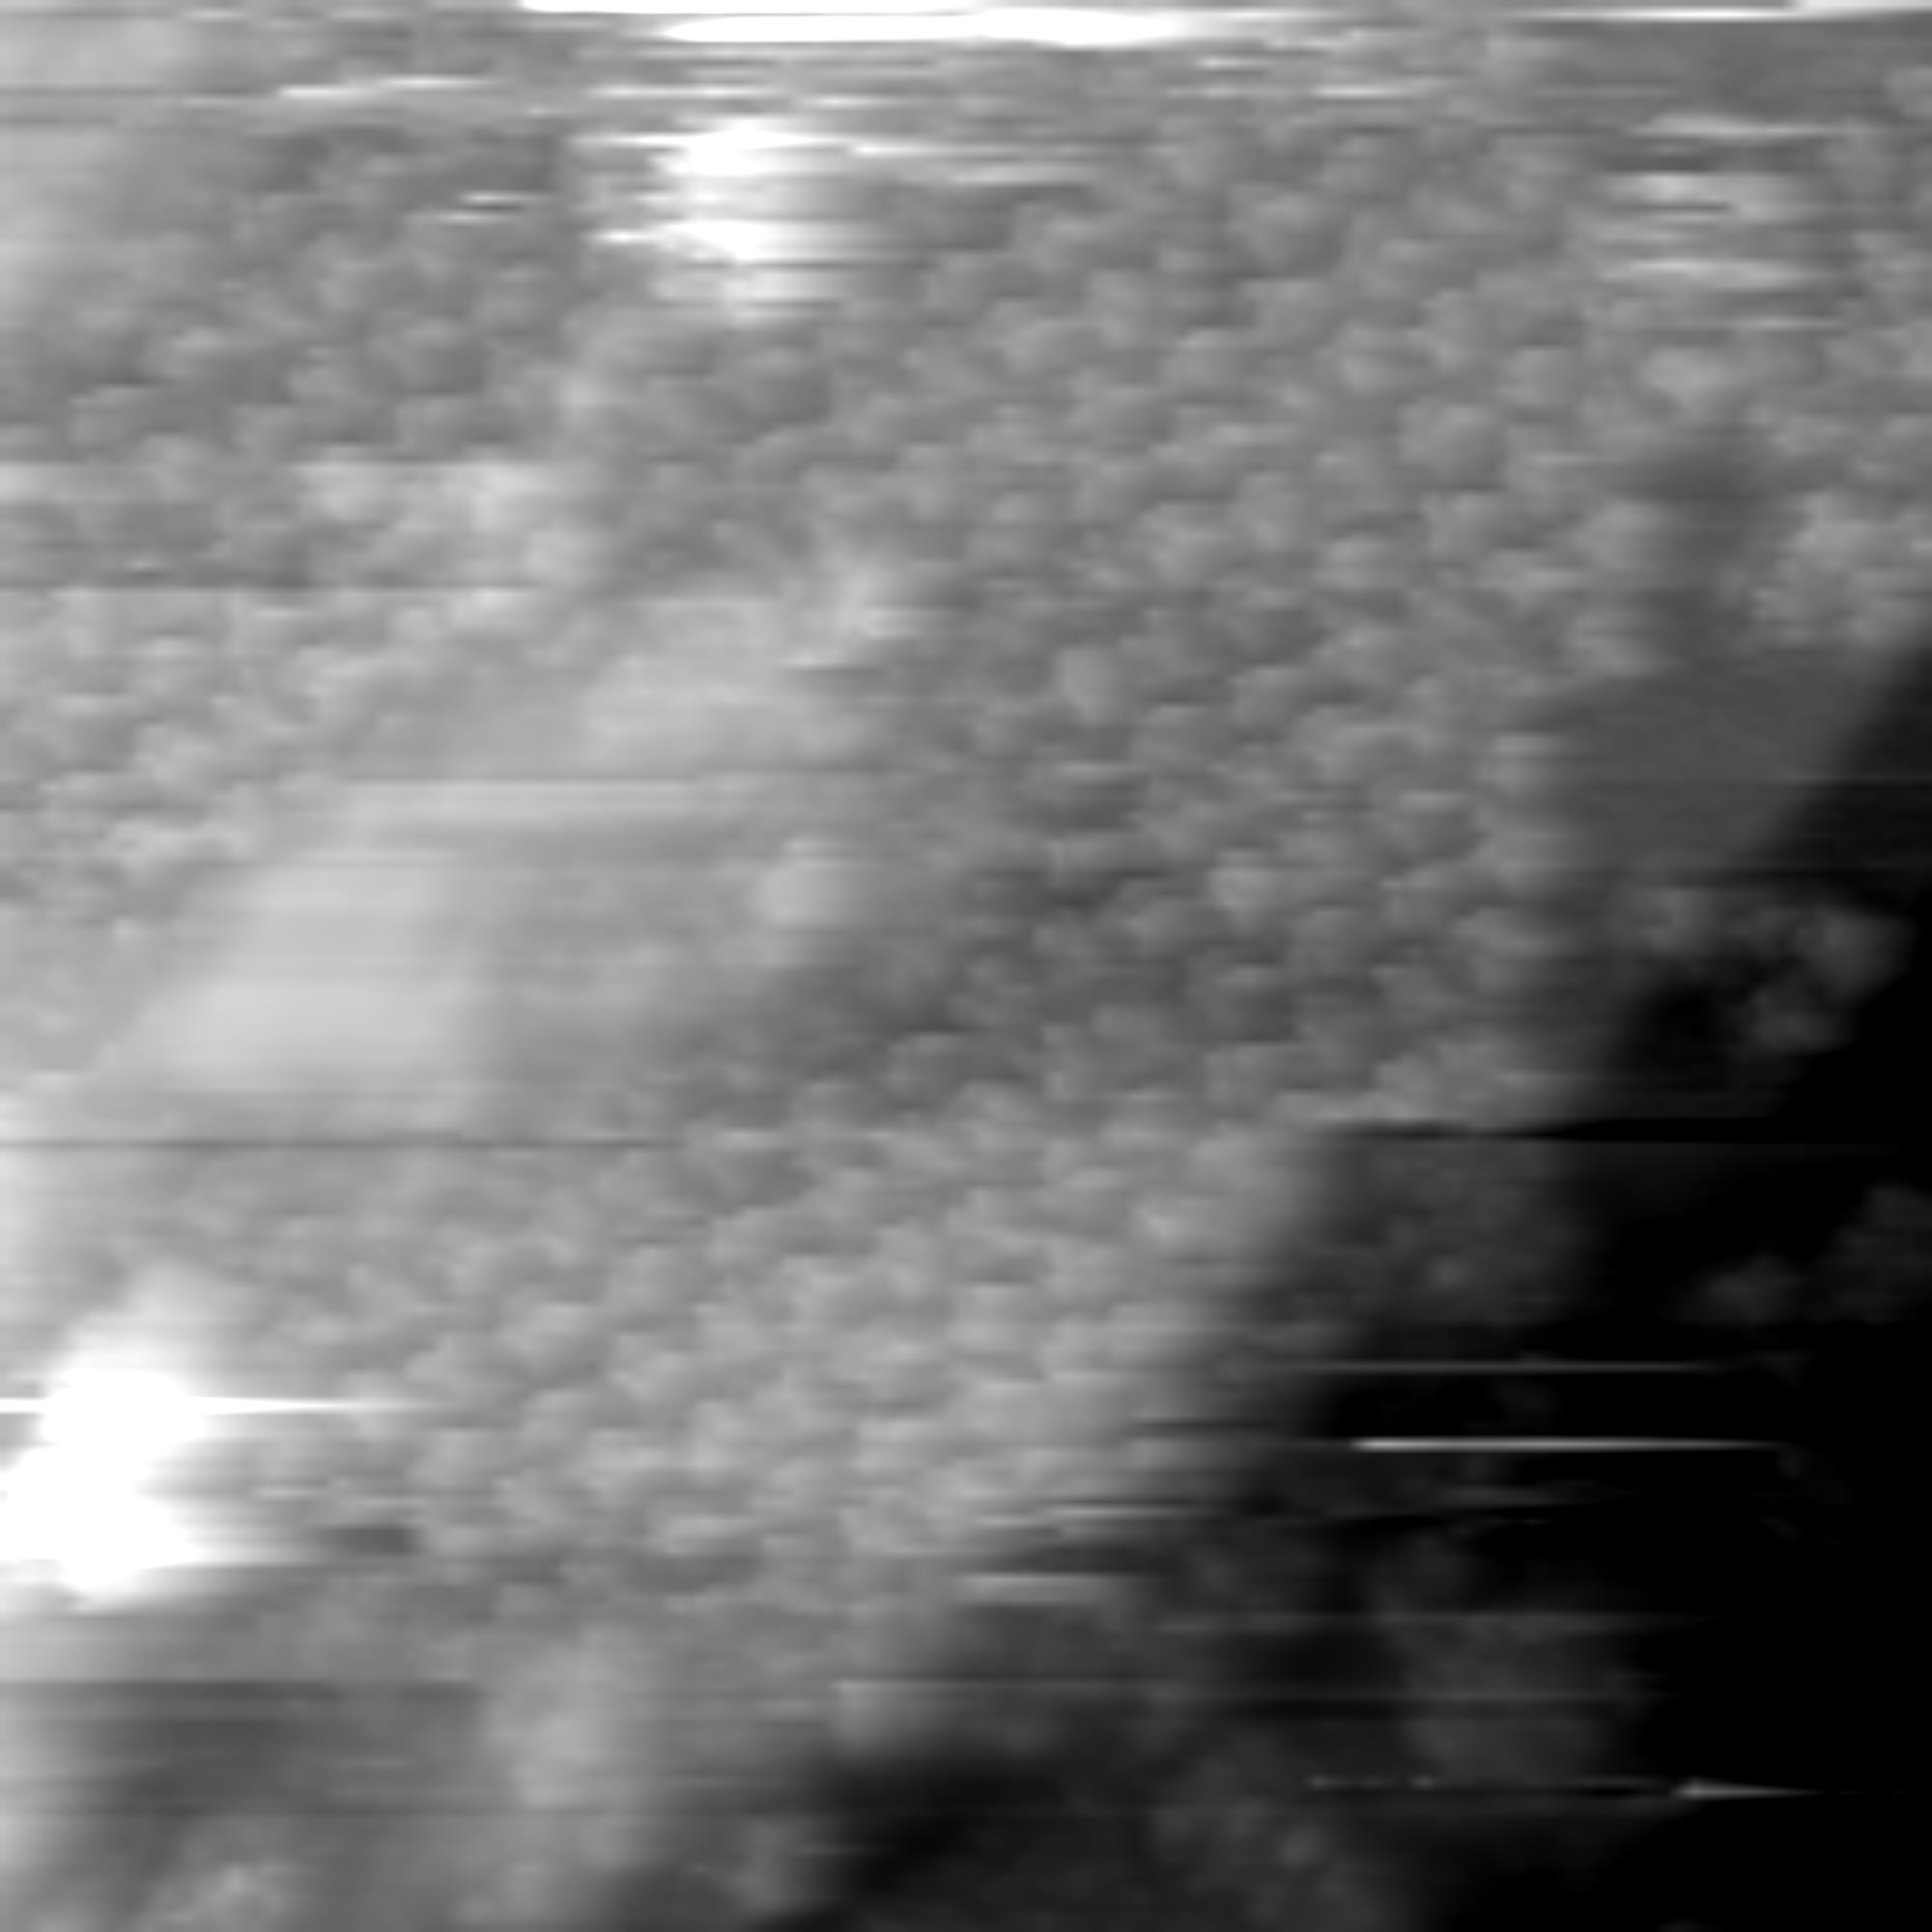
\includegraphics[width=0.5\textwidth]{./images/F151007-112800}
	\caption{TBP on Ag(100) showing some ordering}
	\label{fig:hex-TBP-Ag100}
\end{figure}
%%%%%%%%%%%%%%%%%%%%%%%%%%%%%%%%%%%%%%%%%%%%%%%%%%%%%%%%%%%%%%%%%%%%%%%%%%%%%%%%%%%%%%%%%%%%%%%%%%%
%%%%%%%%%%%%%%%%%%%%%%%%%%%%%%%%%%%%%%%%%%%%%%%%%%%%%%%%%%%%%%%%%%%%%%%%%%%%%%%%%%
	\begin{figure}[]
		\centering
		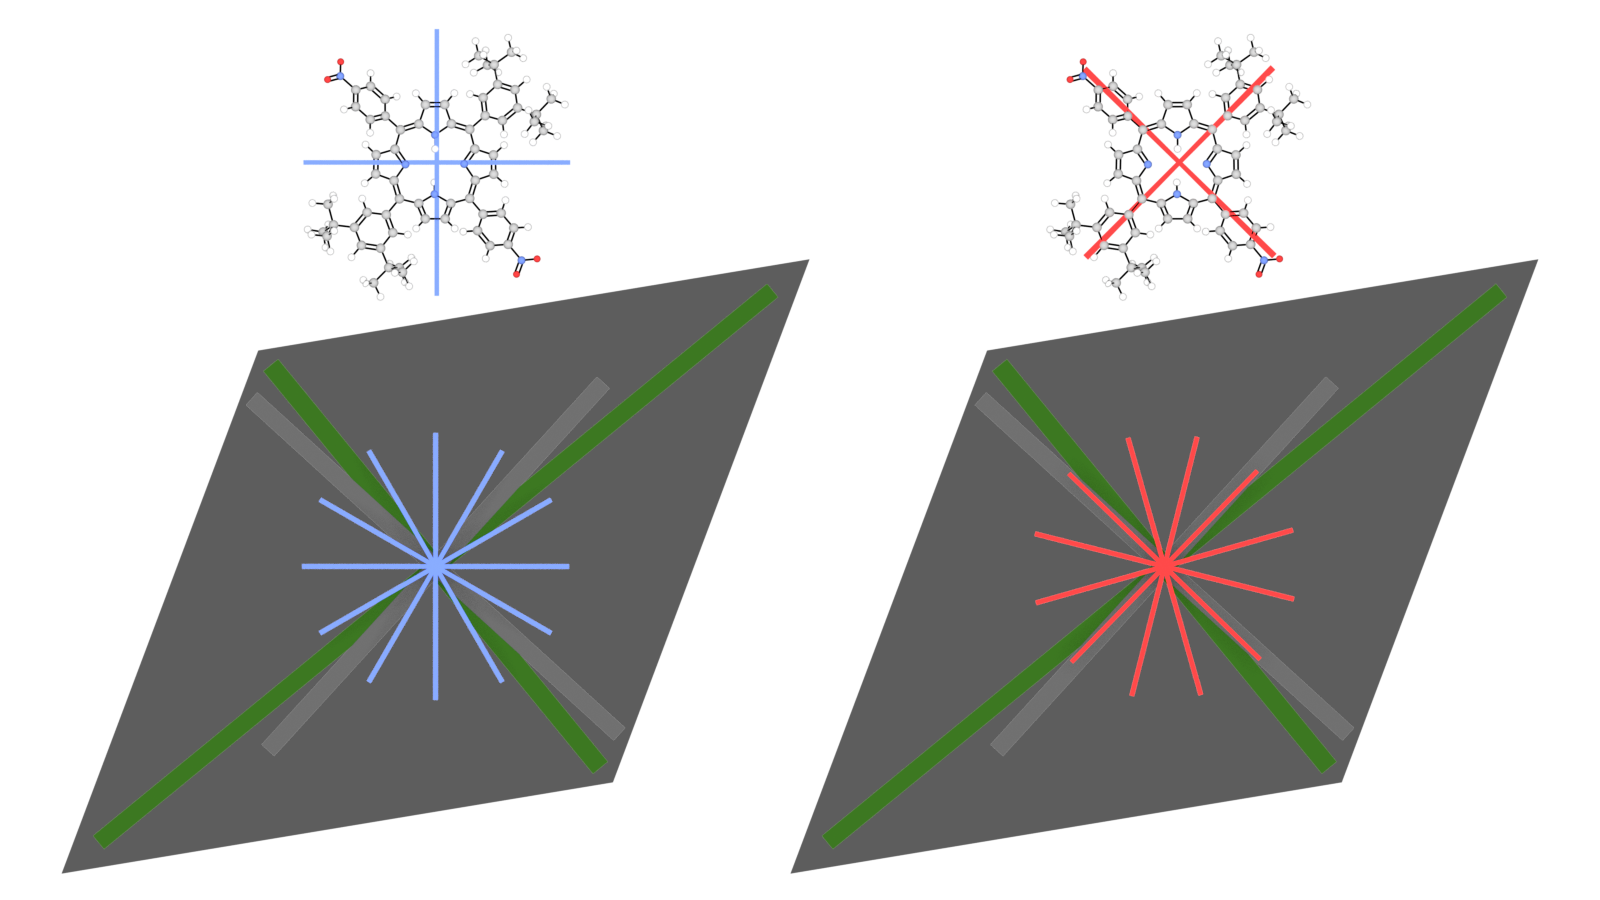
\includegraphics[width=\textwidth]{./images/F160429-185245-R-model-2-crystal-orientation.png}
		\caption{Symmetry relations between TBP molecule and Ag(100) crystal substrate. The same molecular model is highlighted in two different ways, emphasizing the two molecular axis (red/blue). Since the assembly is made up of three different orientations, the three rotated axis sets are shown. The assemblies derived unit cell is shown as shaded background with short and long symmetry axis highlighted in green. The crystal orientation from another preparation on the same single crystal is shown in grey.}
		\label{F160429-185245-R-model-2-crystal-orientation.png}			
	\end{figure}
	\vfill
\restoregeometry